\documentclass[main.tex]{subfiles}

%\usepackage[]{algorithm2e}

\usepackage{algorithmicx}
\usepackage[Algorithm,ruled]{algorithm}
\usepackage{algorithm,algcompatible,amsmath}
\algnewcommand\DESCRIPTION{\item[\textbf{Opis:}]}%
\algnewcommand\INPUT{\item[\textbf{Ulaz:}]}%
\algnewcommand\OUTPUT{\item[\textbf{Izlaz:}]}%

\usepackage{mathtools}

\begin{document}

Genetsko programiranje pripada grupi algoritama evolutivnog izračunavanja (EC, eng. \textit{Evolutionary Computation}) koji su zasnovani na Darvinovoj teoriji evolucije. Tokom 1970-ih, Holand je predložio genetski algoritam kao jedan vid evolutivnog izračunavanja \cite{holland}, dok je njegov učenik Džon Koza 1988. patentirao genetsko programiranje. Tokom 1990-ih i ranih 2000-ih Koza je izdao veliki broj radova i knjiga o genetskom programiranju, od kojih je najznačajnija knjiga \cite{koza} koja predstavlja prvu knjigu iz ove oblasti, a sadrži i princip primene te metode na problem simboličke regresije.

Osnovna ideja genetskih algoritama (GA) i genetskog programiranja (GP) je simulacija procesa evolucije. Prema Darvinu, bolje prilagođene jedinke imaju veću šansu da prežive i putem razmnožavanja prenesu svoj genetski materijal u narednu generaciju. Na taj način, celokupna vrsta se kontinuirano usavršava. Generalno, genetski algoritam se sastoji u iterativnoj popravci inicijalne populacije rešenja koje se često nazivaju jedinke ili hromozomi. Svaka jedinka odgovara jednom rešenju u pretraživačkom prostoru. Jedinke se evaluiraju na osnovu funkcije prilagođenosti. U svakom koraku algoritma, nad jedinkama se primenjuju različiti genetski operatori. Operator selekcije obezbeđuje da verovatnoća sa kojom jedinka prelazi u narednu generaciju zavisi od njene prilagođenosti. Primena operatora ukrštanja i mutacije na selektovane jedinke simulira proces reprodukcije. Razlika između GA i GP je u tome što su jedinke kod GA predstavljene linearnim struktuama poput nizova, dok GP radi nad stabloidnim strukturama. Algoritam \autoref{alg:GPscheme} predstavlja uopštenu šemu genetskog programiranja. Gotovo svi koraci se mogu na veliki broj različitih načina prilagoditi konkretnoj primeni.

\begin{algorithm}
\floatname{algorithm}{Algoritam}
\caption{Osnovna struktura GP metode}
\label{alg:GPscheme}
  \begin{algorithmic}[1]
    \INPUT GP parametri i kriterijum zaustavljanja;
    \OUTPUT najbolja jedinka tj. izraz koji predstavlja rešenje problema;
    \STATE Generisati početnu populaciju jedinki;
    \STATE Izračunati prilagođenost svake jedinke u populaciji;
    \WHILE{nije zadovoljen kriterijum zaustavljanja}
      \STATE Izabrati iz populacije skup jedinki za reprodukciju;
      \STATE Primenom operatora ukrštanja kreirati nove jedinke;
      \IF{ispunjen uslov za mutaciju}
        \STATE Primeniti mutaciju nad novim jedinkama;
      \ENDIF
      \STATE Izračunati prilagođenost novih jedinki;
      \STATE Formirati novu generaciju na osnovu novih jedinki;
    \ENDWHILE
    \STATE \textbf{return} najbolja jedinka;
  \end{algorithmic}
\end{algorithm}

\subsection{Reprezentacija jedinki i generisanje početne populacije}
\label{sec:individual}

Kako jedinka treba da odgovara rešenju problema, u slučaju simboličke regresije pomoću jedne jedinke će biti predstavljen jedan izraz koji je u obliku sintaksnog stabla.

Kao skup funkcija koje se mogu naći u unutrašnjim čvorovima stabla, najčešće se koriste: {+, -, *, /, exp, sin, cos, log}. 

Kao terminali se koriste promenljive definisane na osnovu dostupnog skupa podataka i efemerne slučajne konstante. Efemerna slučajna konstanta je slučajno generisani broj određenog tipa iz definisanog intervala. Kod problema čije su nezavisne promenljive realni brojevi, prirodno je odabrati da efemerne konstante takođe budu realnog tipa i da budu iz nekog prikladnog opsega (često je to [-1, 1]) \cite{koza}.

Početna populacija jedinki se generiše na slučajan način. Taj proces se može implementirati na više različitih načina, čime se postiže formiranje inicijalnih stabala različitih veličina i oblika. Dva osnovna načina su "full" i "grow" metode \cite{koza}.  

Oba pristupa se zasnivaju na dubini stabla. Dubina stabla se definiše kao put od korena do najudaljenijeg lista.

"Full" metoda podrazumeva generisanje potpunog stabla, tj. stabla kod koga je put između korena i svakog lista jednak definisanoj maksimalnoj dubini. Ovo se postiže ograničavanjem izbora vrste čvora u zavisnosti od trenutne dubine. Ako se trenutni čvor koji se generiše nalazi na dubini koja je manja od maksimalne, može se izabrati samo čvor koji predstavlja funkciju. U suprotnom, ako se trenutni čvor koji se generiše nalazi na dubini koja je jednaka maksimalnoj, onda se može odabrati samo terminal.

"Grow" metoda podrazumeva generisanje stabala čiji oblici variraju. Od značaja je samo da dužina puta od korena do bilo kog lista ne bude veća od definisane maksimalne dubine, a dozvoljeno je da bude kraća. Ako se trenutni čvor koji se generiše nalazi na dubini koja je manja od maksimalne, može se izabrati ili čvor koji predstavlja funkciju ili čvor koji predstavlja terminal, pri čemu se izbor vrši na slučajan način. Ako se trenutni čvor koji se generiše nalazi na dubini koja je jednaka maksimalnoj, onda se može odabrati samo terminal. 

Kod obe metode važi sledeće: Ako je trenutni čvor koji se generiše na dubini koja je manja od minimalne, moguće je odabrati samo funkciju.

Na osnovu \cite{koza}, najbolji pristup generisanju inicijalne populacije bila bi "ramped half-and-half" metoda koja omogućava da se kreira širok spektar stabala različitih visina i oblika. Ona predstavlja kombinaciju "full" i "grow" metoda. Takođe, obezbeđuje i kreiranje podjednakog broja stabala po svakom nivou dubine od nivoa 2 do nivoa definisanog parametrom maksimalne dubine. Na primer, ako je definisana maksimalna dubina jednaka 6, onda će 20\% stabala imati dubinu 2, 20\% dubinu 3, ..., 20\% dubinu 6. Dalje, za svaki nivo dubine 50\% stabala se kreira pomoću "full", a 50\% pomoću "grow" metode.


\subsection{Funkcija prilagođenosti}
\label{sec:fitness}

Funkcija prilagođenosti (eng. \textit{fitness function}) daje ocenu kvaliteta jedinke i utiče na verovatnoću izbora te jedinke za proces formiranja nove generacije. Svakoj jedinki je pridružena skalarna vrednost koja predstavlja njenu prilagođenost i rezultat je neke eksplicitno definisane funkcije. Ta funkcija npr. može biti MSE greška na skupu podataka za trening i u tom slučaju prilagođenije jedinke imaju manju vrednost fitnes funkcije.

U knjizi \cite{koza}, Koza definiše 4 vrste funkcija prilagođenosti:
\begin{itemize}
    \item "Raw" funkcija prilagođenosti (eng. \textit{raw fitness}) % smisliti prevod
    \item Standardizovana funkcija prilagođenosti (eng. \textit{standardized fitness})
    \item "Adjusted" funkcija prilagođenosti (eng. \textit{adjusted fitness})
    \item Normalizovana funkcija prilagođenosti (eng. \textit{normalized fitness})
\end{itemize}

Definicije ovih funkcija nisu međusobno isključive, već se svaka od funkcija definiše na osnovu prethodno uvedene.

\subsubsection{"Raw" funkcija prilagođenosti}
\label{sec:rawFitness}

"Raw" funkcija prilagođenosti se izražava u terminima problema koji se rešava. Kod simboličke regresije "raw" funkcija prilagođenosti se može posmatrati kao funkcija greške. Njena vrednost za neku jedinku odgovara zbiru distanci izmedju vrednosti koje daje izraz predstavljen tom jedinkom i pravih ciljnih vrednosti svih uzoraka iz trening skupa. Distanca se računa kao apsolutna vrednost razlike između predviđenih i pravih vrednosti. Formalno, "raw" funkcija prilagođenosti $r(i,t)$ za $i$-tu jedinku iz generacije $t$ se računa kao

\[ r(i,t) = \sum_{i=1}^{N}|y_i - \hat{y_i}|  \]
gde je N broj uzoraka u trening skupu, $y_i$ prava vrednost cljne promenljive, a $\hat{y_i}$ predviđena vrednost cljne promenljive pomoću $i$-te jedinke.

U zavisnosti od definicije problema, prilagođenije jedinke mogu imati ili manju ili veću $r(i,t)$ vrednost.
Pošto "raw" prilagođenost kod simboličke regresije odgovara grešci, onda bolje jedinke imaju manju vrednost date funkcije.


\subsubsection{Standardizovana funkcija prilagođenosti}
\label{sec:rawFitness}

Standardizovana funkcija prilagođenosti $s(i,t)$ redefiniše "raw" funkciju tako da njena vrednost za bolje jedinke uvek bude manja, bez obzira na vrstu problema koji se rešava. 

Kako je kod simboličke regresije "raw" funkcija već definisana tako da manje vrednosti reprezentuju bolje jedinke, standardizovana funkcija će biti jednaka "raw" funkciji. Odnosno,

\[ s(i,t) = r(i,t). \]

Kod problema kod kojih je "raw" prilagođenost definisana tako da se boljim jedinkama smatraju one sa većom vrednošću te funkcije, standardizovana funkcija bi bila jednaka razlici maksimalne moguće vrednosti "raw" funkcije (označene sa $r_{max}$) i vrednosti "raw" funkcije za datu jedinku

\[ s(i,t) = r_{max} - r(i,t). \]


\subsubsection{"Adjusted" funkcija prilagođenosti}
\label{sec:adjustedFitness}

"Adjusted" funkcija prilagođenosti $a(i,t)$ se računa na osnovu standardizovane funkcije na sledeći način

\[ a(i,t) = \frac{1}{1 + s(i,t)}. \]

Vrednost $a(i,t)$ pripada intervalu [0,1] i veća je za bolje jedinke.

Prednost ove funkcije prilagođenosti je u tome što naglašava razliku između dobrih i vrlo dobrih jedinki. Na primer, ako imamo dve loše jedinke čije su vrednosti standardizovane funkcije redom 64 i 65, njihove vrednosti prilagođene funkcije će biti 0.0154 i 0.0156. U oba slučaja, razlika između prilagođenosti ove dve loše jedinke nije velika. A ako imamo dve dobre jedinke čije su vrednosti standardizovane funkcije redom 4 i 3, njihove vrednosti prilagođene funkcije će biti 0.20 i 0.25. %Ovde, iako su jedinke na osnovu vrednosti standardizovane funkcije bliske, na osnovu prilagođene funkcije dodatno se ističe bolja jedinka udaljivši se od svog suseda.
Ovde, iako su jedinke na osnovu vrednosti standardizovane funkcije bliske, na osnovu "adjusted" funkcije se dodatno ističe bolja od dve posmatrane dobre jedinke.

\subsubsection{Normalizovana funkcija prilagođenosti}
\label{sec:normalizedFitness}

Normalizovana funkcija prilagođenosti $n(i,t)$ se računa na osnovu prilagođene funkcije na sledeći način

\[ n(i,t) = \frac{a(i,t)}{\sum_{k=1}^{M}a(k,t)}, \]
gde je M veličina populacije.

Odnosno, za jedniku $i$ "adjusted" funkcija prilagođenosti se normalizuje u skladu sa "adjusted" funkcijama ostalih jedinki iz populacije.

Normalizovana funkcija prilagođenosti ima tri poželjne karakteristike:

\begin{itemize}
    \item Njena vrednost pripada intervalu [0, 1].
    \item Veća je za bolje jedinke u populaciji.
    \item Zbir normalizovanih vrednosti prilagođenosti svih jedinki je jednak 1.
\end{itemize}

Nedostatak ove vrste funkcije prilagođenosti jeste u tome što se u populaciji može nalaziti neka jedinka čiji izraz nije definisan nad svim tačkama iz skupa podataka, pa će to uticati i na vrednost funkcije prilagođenosti ostalih jedinki. Naime, ako neka jedinka nije definisana nad svim tačkama iz skupa podataka, vrednost njene "raw" funkcije će takođe biti nedefinisana, a samim tim i vrednost "adjusted" funkcije. A to će onemogućiti izračunavanje normalizovane funkcije prilagođenosti čak i za neku drugu jedinku koja je definisana nad svim tačkama. %Zbog toga će u ovom radu biti korišćena "adjusted" funkcija prilagođenosti.

U ovom radu će biti korišćena "adjusted" funkcija prilagođenosti, po ugledu na \cite{koza}.



\subsection{Selekcija}
\label{sec:selection}

Selekcija obezbeđuje čuvanje i prenošenje dobrih osobina populacije (tj. dobrog genetskog materijala) na sledeću generaciju. U svakoj generaciji, deo jedinki se izdvaja za reprodukciju i generisanje nove generacije. Izdvajanje jedinki koje će učestvovati u reprodukciji zasniva se na funkciji prilagođenosti i, generalno, prilagođenije jedinke imaju veću verovatnoću da budu izabrane. 

Proces selekcije se može realizovati putem ruletske selekcije, turnirske selekcije, rangiranjem prema funkciji prilagođenosti ili na neki drugi način. U ovom radu je primenjena turnirska selekcija koja funkcioniše na sledeći način. Iz tekuće populacije se na slučajan način bira unapred zadati broj jedinki. Taj broj je određen parametrom $k$ koji predstavlja veličinu turnira. Od izabranih $k$ jedinki se zatim bira najbolje prilagođena jedinka. Time se i slabije prilagođenim jedinkama daje određena šansa da budu izabrane za reprodukciju.

\subsection{Operatori ukrštanja}
\label{sec:crossover}

Za potrebe rešavanja problema simboličke regresije razvijani su različiti operatori ukrštanja. %U ovom radu će biti predstavljene dve vrste operatore: standardni operator ukrštanja i operatori ukrštanja zasnovani na semantici.
U ovom radu će biti predstavljene dve varijante genetskog programiranja - jedna koja koristi standardni operator uktštanja i druga koja koristi operator ukrštanja zasnovan na semantičkoj sličnosti.

\subsubsection{Standardni operator ukrštanja}
\label{sec:stdCrossover}

Operator ukrštanja (eng. \textit{crossover}) se koristi u procesu reprodukcije u kom učestvuju jedinke izabrane procesom selekcije. U ukrštanju učestvuju dve jedinke koje se nazivaju roditeljima. Rezultat ukrštanja su dve nove jedinke koje se nazivaju decom ili neposrednim potomcima. Očekivano je da deca nasleđuju osobine roditelja, uključujući njihovu prilagođenost, pa i da imaju bolju prilagođenost od njih.

Kod simboličke regresije, ukrštanje dve jedinke podrazumeva razmenu njihovih slučajno odabranih podstabala. Kod oba roditelja se odabere po jedan čvor, slučajnim izborom iz uniformne raspodele, koji će predstavljati tačku ukrštanja. Fragment ukrštanja svakog roditelja je podstablo određeno tim čvorom kao korenom i svim čvorovima koji se nalaze ispod njega. Zatim je potrebno samo razmeniti odabrane fragmente između te dve jedinke. 

Primer standardnog ukrštanja se može videti na slici \ref{fig:standardCrossover}.
Na slikama (a) i (b) su prikazane dve jedinke koje su odabrane za proces ukrštanja i na svakoj od njih su obeleženi čvorovi koji predstavljaju tačku ukrštanja, kao i podstabla određena tim čvorovima. Na slikama (c) i (d) su prikazane dve jedinke koje nastaju nakon razmene podstabala definisanih izabranim tačkama ukrštanja.

\begin{figure}[!ht]
\begin{center}
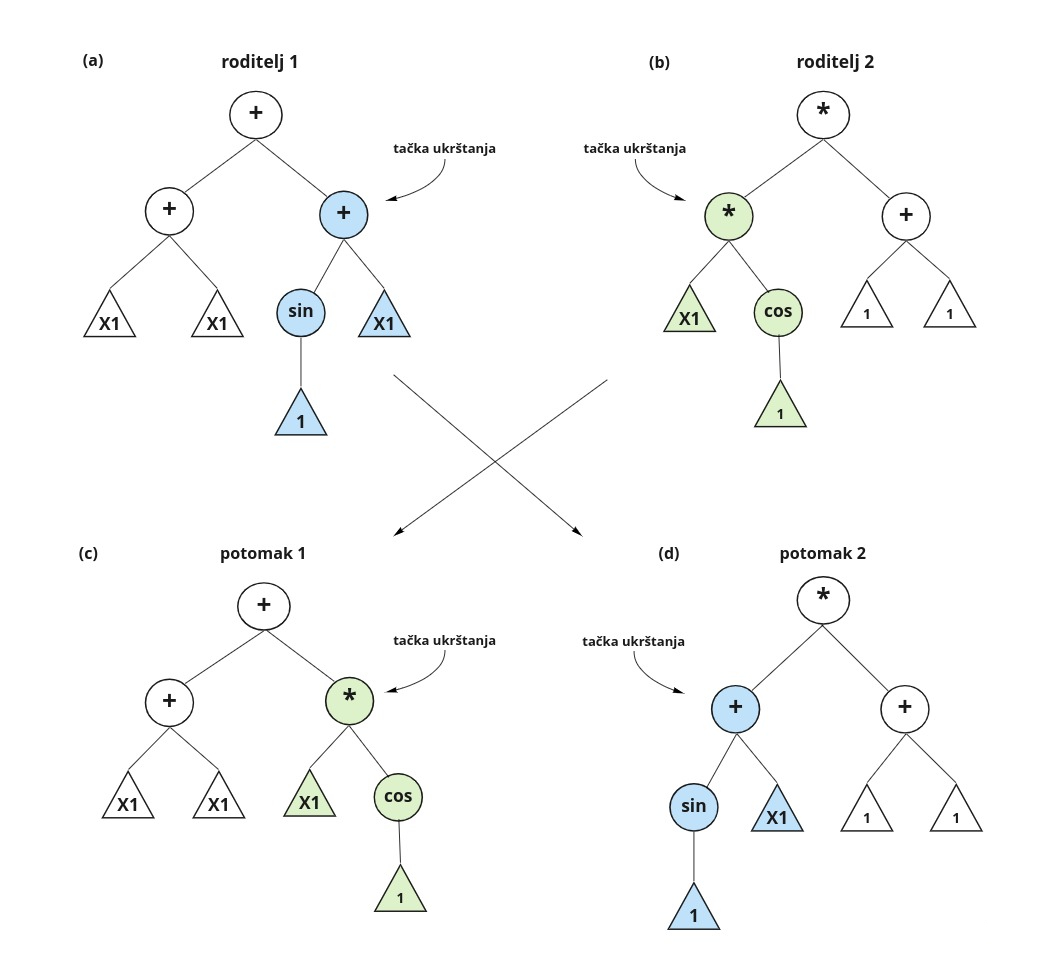
\includegraphics[width=0.9\textwidth]{../images/standard_crossover4.jpg}
\end{center}
\caption{Primer standardnog ukrštanja dva stabla}
\label{fig:standardCrossover}
\end{figure}

Treba imati u vidu da su jedinke koje su odabrane za ukrštanje obično različite veličine i da se vrlo brzo može desiti da jedinke koje nastaju ukrštanjem dostignu ogromne razmere (npr. slučajevima kada se u jednom stablu kao čvor ukrštanja izabere terminal, a u drugom stablu čvor koji određuje visoko podstablo). Kako bi se ovo onemogućilo, uveden je parameter kojim se ograničava veličina jedinki koje nastaju ukrštanjem. Ako se formira jedinka nedozvoljene veličine, umesto nje će u narednu generaciju ići jedan od roditelja.


\subsubsection{Operatori ukrštanja zasnovani na semantici}
\label{sec:semanticallyBasedCrossover}

Pored osnovnog operatora ukrštanja, tokom godina su razvijani i drugi pristupi koji bi dali kvalitetnije jedinke. Neki od njih su i operatori ukrštanja koji su zasnovani na semantici \cite{semanticCrossover}.

Semantika nekog podstabla se aproksimira pomoću vrednosti dobijenih evaluacijom tog podstabla na predefinisanom skupu tačaka iz domena problema. Ovo se naziva \textit{semantikom uzorkovanja} (SS, eng. \textit{Sampling Semantics}).
Formalno, \textit{semantika uzorkovanja} nekog stabla (ili podstabla) se definiše na sledeći način:

Neka je $F$ funkcija koja je izražena pomoću (pod)stabla $T$ na domenu $D$ i neka je $P$ skup tačaka iz domena $D$, $P = \{p_1, p_2, ..., p_N\}$. Tada je \textit{semantika uzorkovanja} stabla $T$ na skupu $P$ u domenu $D$, skup $S = \{s_1, s_2, ..., s_N\}$ takav da je $s_i = F(p_i), i=1,2,..,N$.

Vrednost broja $N$ zavisi od problema. Ako se u skupu podataka nalazi veoma malo tačaka, SS može biti neprecizna, a ako ih ima mnogo, izračunavanje SS može biti vremenski zahtevno. Izbor tačaka $P$ je takođe bitan. Ako su tačke suviše bliske skupu funkcija koje se koriste u GP (npr. $\pi$ za trigonometrijske funkcije, $e$ za logaritamske funkcije), semantika može biti pogrešno protumačena. Zbog toga se skup $P$ bira na slučajan način.

Na osnovu SS definiše se \textit{rastojanje semantike uzorkovanja} (SSD, \textit{Sampling Semantics Distance}) između dva podstabla. Neka je $P = \{p_1, p_2, ..., p_N\}$ \textit{semantika uzorkovanja} podstabla $St_1$, a $Q = \{q_1, q_2, ..., q_N\}$ \textit{semantika uzorkovanja} podstabla $St_2$. Onda se $SSD$ između $St_1$ i $St_2$ definiše kao

\[ SSD(St_1, St_2) = \frac{1}{N}(|p_1 - q_1| + |p_2 - q_2| + ... + |p_N - q_N|). \]

Pomoću $SSD$ se mogu definisati dve vrste semantičkih veza između podstabala - \textit{semantička ekvivalentnost} i \textit{semantička sličnost}.

Dva podstabla su \textit{semantički ekvivalentna} (SE, eng. \textit{Semantically Equivalent}) na domenu ako je njihova $SSD$ vrednost dovoljno mala

\[
    SE(St_1, St_2)= 
\begin{dcases}
    true,& \text{ako je } SSD(St_1, St_2) < \epsilon\\
    false,              & \text{inače}
\end{dcases}
\]
                        
Parametar $\epsilon$ predstavlja \textit{semantičku osetljivost} (eng. \textit{semantic sensitivity}). Na osnovu eksperimenata iz \cite{SACanalysis}, za $\epsilon$ je najbolje uzeti neku vrednost iz skupa \{0.01, 0.02, 0.04, 0.05, 0.06, 0.08, 0.1\}.

Dva podstabla su \textit{semantički slična} ($SS_i$, eng. \textit{Semantically Similar}) na domenu ako njihova $SSD$ vrednost leži na nekom pozitivnom intervalu:

\[
    SS_i(St_1, St_2)= 
\begin{dcases}
    true,& \text{ako je } \alpha < SSD(St_1, St_2) < \beta\\
    false,              & \text{inače}
\end{dcases}
\]
gde su $\alpha$ i $\beta$ donja i gornja granica semantičke osetljivosti (LBSS, eng. \textit{Lower Bound Semantic Sensitivity} i UBSS, eng. \textit{Upper Bound Semantic Sensitivity}). Najbolje vrednosti za ove parametre variraju od problema do problema. U radu \cite{semanticCrossover} se pokazalo da su za simboličku regresiju, nad jednačinama koje su korišćene i u ovom radu, najbolje rezultate dale vrednosti između 0.4 i 0.6 za $UBSS$, a vrednosti $10^{-2}$ ili manje za $LBSS$.

Intuicija korišćenja semantičke sličnosti je u tome što je verovatnije da će razmena podstabala biti korisnija ukoliko se odvija između dve jedinke koje nisu semantički identične, ali nisu ni semantički suviše različite. Motivacija za ovo je uzeta iz bioloških procesa i sličnosti MHC gena (koji imaju ulogu u imunom odgovoru) između dve jedinke. Za potomke je najbolje kada one imaju različite MHC gene, ali ne previše različite.\\


\textbf{Operator ukrštanja koji je svestan semantike}
\\

Operator ukrštanja koji je svestan semantike (SAC, eng. \textit{Semantics Aware Crossover}) je prvobitno predložen u radu \cite{SAC}. Motivacija za uvođenje ovog operatora je bila mogućnost razmene semantički ekvivalentnih podstabala kod običnog operatora ukrštanja zasnovanog na slučajnom izboru, što rezultuje kreiranjem potomaka koji su identični svojim roditeljima. Na primer, ako su data dva stabla kao na slici \ref{fig:sac1} i ako su za razmenu odabrana označena podstabla, onda će kao rezultat ukrštanja nastati stabla kao na slici \ref{fig:sac2} . Iako su sintaksno različita, podstabla koja su izabrana za razmenu su semantički ekvivalentna (oba imaju semantiku $2X$). Ovakvim ukrštanjem ništa nije postignuto - u populaciji i dalje ostaju dva stabla koja imaju istu vrednost funkcije prilagođenosti.


\begin{figure}[!ht]
\begin{center}
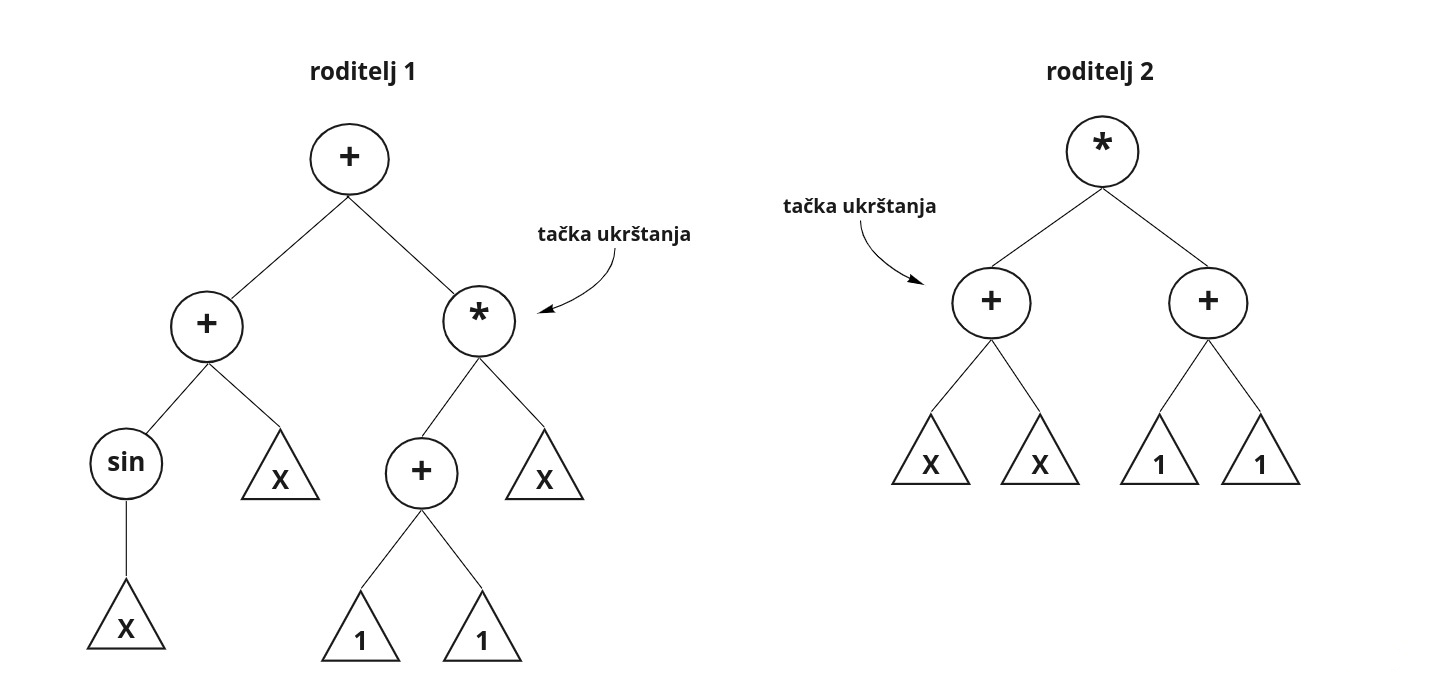
\includegraphics[width=0.7\textwidth]{../images/SAC1.jpg}
\end{center}
\caption{Selekcija semantički ekvivalentnih podstabala}
\label{fig:sac1}
\end{figure}

\begin{figure}[!ht]
\begin{center}
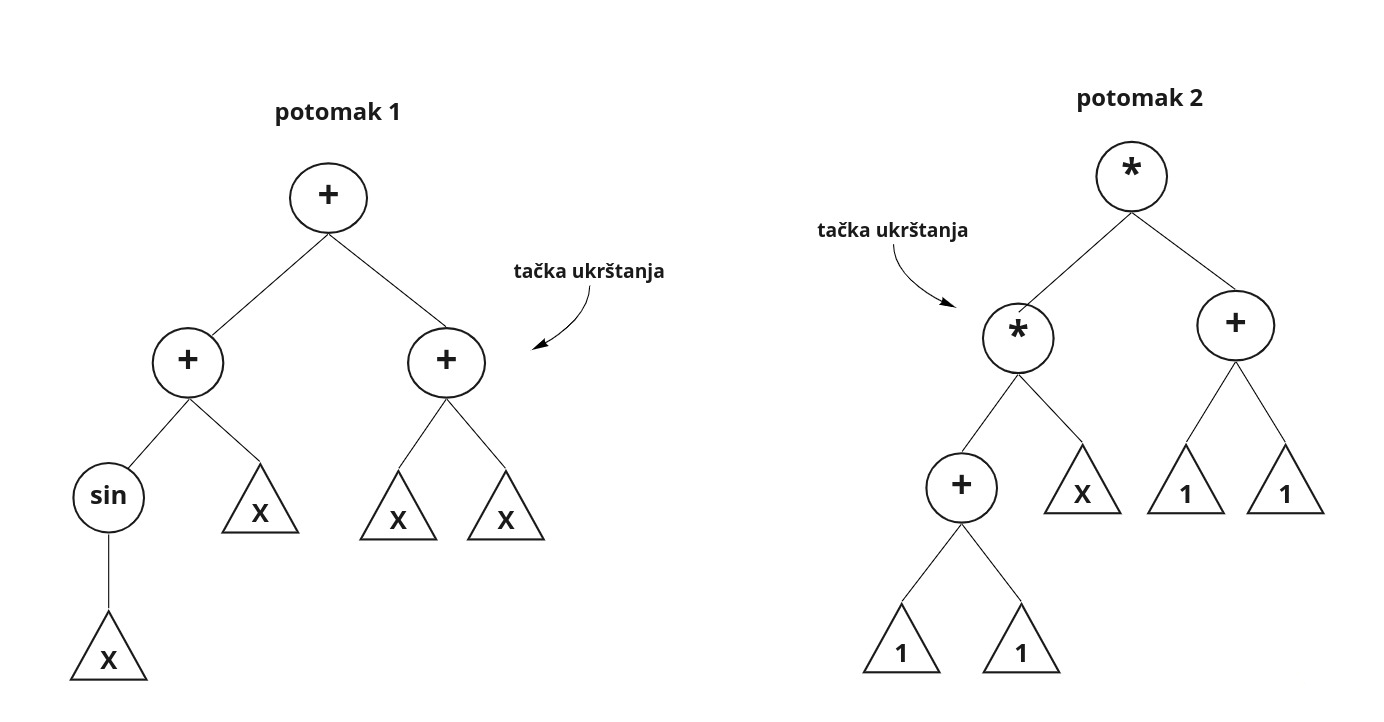
\includegraphics[width=0.7\textwidth]{../images/SAC2.jpg}
\end{center}
\caption{Deca generisana ukrštanjem semantički ekvivalentnih podstabala}
\label{fig:sac2}
\end{figure}

SAC sprečava razmenu ovakvih, semantički ekvivalentnih, podstabala. Svaki put kada se odaberu dva podstabla za razmenu, proverava se njihova ekvivalentnost pomoću formule za $SE$. Ako su ekvivalentna, ponovo se na slučajan način biraju tačke ukrštanja. \\

\textbf{Operator ukrštanja koji je zasnovan na semantičkoj sličnosti}
\\

Operator ukrštanja koji je zasnovan na semantičkoj sličnosti (SSC, eng. \textit{Semantic Similarity-based Crossover}) predstavlja proširenje SAC operatora. Kod ove metode ukrštanja, kada se odaberu podstabla, umesto semantičke ekvivalencije, proverava se njihova semantička sličnost. Pošto je semantičku sličnost mnogo teže zadovoljiti u odnosu na semantičku ne-ekvivalentnost, verovatno je da će doći do uzastopnih neuspešnih pokušaja potrage za takvim podstablima. Zbog toga, SSC metoda koristi veći broj pokušaja da nađe semantički sličan par, a okreće se ka slučajnom izboru ako pređe dozvoljeni broj pokušaja. Algoritam \autoref{alg:ssc} prikazuje SSC metodu.

\\

\begin{algorithm}
\floatname{algorithm}{Algoritam}
\caption{Algoritam ukrštanja zasnovanog na semantičkoj sličnosti}
\label{alg:ssc}
  \begin{algorithmic}[1]
    \INPUT $skupJedinki$ - skup jedinki iz kog je potrebno izabrati dve jedinke za ukrštanje, $\alpha$ - donja granica semantičke osetljivosti, $\beta$ - gornja granica semantičke osetljivosti, $maxBrojPokusaja$ - maksimalan broj pokušaja odabira semantički sličnog para jedinki
    \OUTPUT;
    \STATE Izabrati roditelja $P_1$ iz $skupaJedinki$;
    \STATE Izabrati roditelja $P_2$ iz $skupaJedinki$;
    \STATE $brojPokusaja = 0$;
    \WHILE{$brojPokusaja < maxBrojPokusaja$}
      \STATE Na slučajan način izabrati podstablo $St_1$ u roditelju $P_1$;
      \STATE Na slučajan način izabrati podstablo $St_2$ u roditelju $P_2$;
      \STATE Na slučajan način generisati skup tačaka $P$ iz domena $D$;
      \STATE Izračunati $SSD$ između $St_1$ i $St_2$ na tačkama $P$;
      %\IF{$St_1$ je slično $St_2$}
      \IF{$\alpha < SSD($St_1$, $St_2$) < \beta$}
        \STATE \color{gray}// \textit{$St_1$, $St_2$ su semantički slični}
        \STATE \color{black}Izvršiti ukrštanje;
        \STATE Dodati decu u novu populaciju;
        \STATE \textbf{return} true;
      \ENDIF
      \STATE $brojPokusaja = brojPokusaja + 1$
    \ENDWHILE
    \IF{$brojPokusaja == maxBrojPokusaja$}
        \STATE Na slučajan način izabrati podstablo $St_1$ u roditelju $P_1$;
        \STATE Na slučajan način izabrati podstablo $St_2$ u roditelju $P_2$;
        \STATE Izvršiti ukrštanje;
        \STATE \textbf{return} true;
      \ENDIF
  \end{algorithmic}
\end{algorithm}



\subsection{Operatori mutacije}
\label{sec:mutation}

Mutacija se primenjuje nakon procesa ukrštanja. Operator mutacije sa određenom (obično veoma malom) verovatnoćom menja jedan deo jedinke na određeni način. Uloga mutacije je da spreči da jedinke u populaciji postanu suviše slične i da pomogne u obnavljanju izgubljenog genetskog materijala. Time sprečava konvergenciju ka lokalnom ekstremumu i omogućava razmatranje novih delova prostora pretrage u kojima se možda nalazi globalni ekstremum. Dovoljno je da se jedna jedinka približi globalnom ekstremumu pa da kroz nekoliko generacija veliki broj jedinki bude u tom delu prostora pretrage.

Postoje različiti načini mutacije stabloidnih jedinki. Neki od njih su mutacija pojedinačnih čvorova stabla i mutacija celog podstabla \cite{ziprian}.

Mutacija pojedinačnog čvora (eng. \textit{point mutation}) podrazumeva zamenu odabranog čvora nekim drugim čvorom. Terminal može biti zamenjen drugim slučajno izabranim terminalom, a funkcija može biti zamenjena drugom funkcijom iste arnosti.

Mutacija celog podstabla (eng. \textit{subtree mutation}) obuhvata slučajni izbor čvora koji će predstavljati koren podstabla koje treba zameniti, generisanje novog stabla na slučajan način i njegovo postavljanje na mesto odabranog podstabla.

Na slici \ref{fig:mutation} se može videti primer obe vrste mutacije. Na slici (a) je predstavljeno originalno stablo nad kojim treba da se izvrši mutacija. Zelenom bojom  obeležen je čvor koji predstavlja izabranu tačku mutacije. Na slici (b) je prikazano stablo koje nastaje kao rezultat primene mutacije pojedinačnog čvora, a na slici (c) stablo koje nastaje kao rezultat primene mutacije celog podstabla.

\begin{figure}[!ht]
\begin{center}
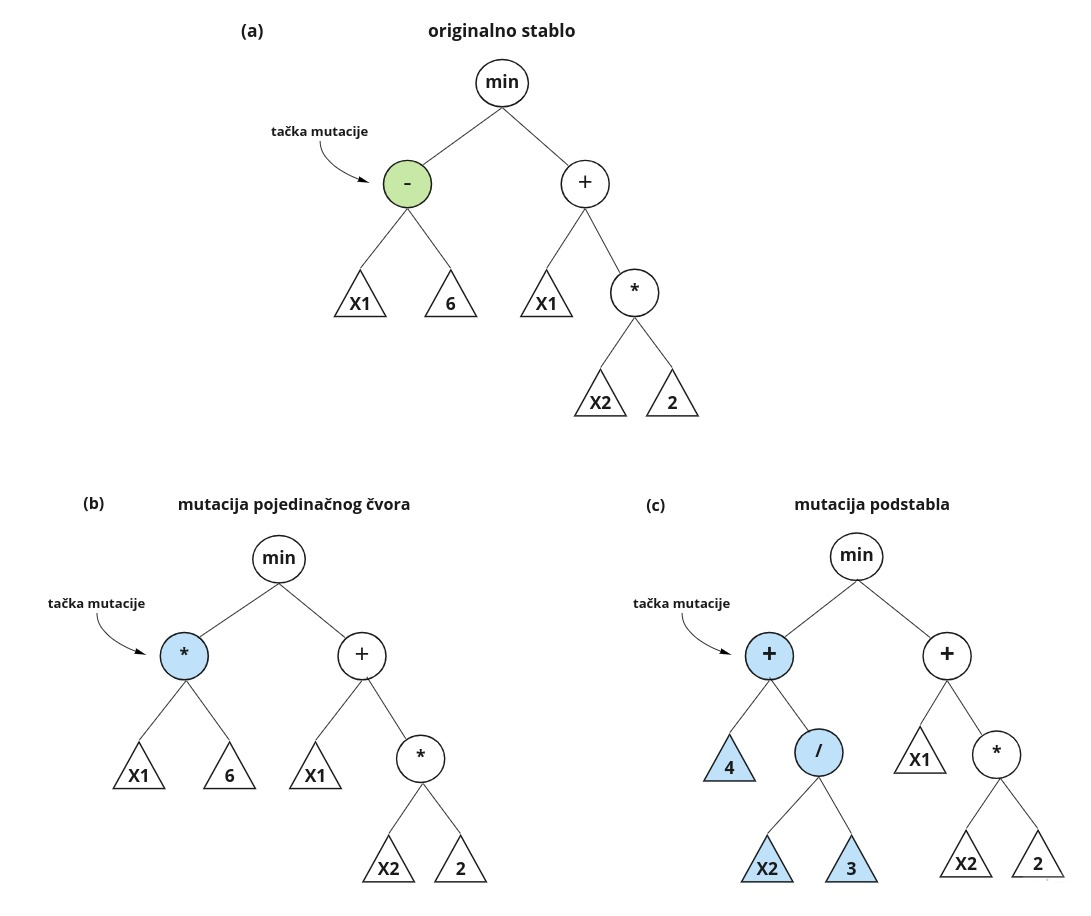
\includegraphics[width=0.95\textwidth]{../images/mutation4.jpg}
\end{center}
\caption{Primer dve vrste mutacije stabla}
\label{fig:mutation}
\end{figure}


\subsection{Zaustavljanje}
\label{sec:stopCondition}

Evolutivni proces stvaranja novih generacija se ponavlja sve dok nije zadovoljen neki uslov zaustavljanja \cite{VI}:

\begin{enumerate}
    \item Pronađeno je rešenje koje zadovoljava unapred zadati kriterijum.
    \item Dostignut je zadati broj generacija.
    \item Dostignut je definisani vremenski kriterijum zaustavljanja.
    \item Funkcija prilagođenosti je izračunata zadati broj puta.
\end{enumerate}

U ovom radu su korišćeni uslovi 1, 2 i 3. u navedenom redosledu, pri čemu se u uslovu 1. smatra da je pronađeno zadovoljavajuće rešenje ako mu je "adjusted" funkcija prilagođenosti veća od 0.9. 



\end{document}